\documentclass{article}
\usepackage[italian]{babel}

\usepackage{epigraph}
\usepackage{fontspec}
\usepackage{graphicx}
\usepackage[hidelinks]{hyperref}
\usepackage{verbatim}
\usepackage{graphicx}

\graphicspath{ {./images/} }

\title{
	\textbf{
		Rapporto del team 13 \\
	}
	\textbf{\large
		Birdazzone \break
		(progetto per l'insegnamento \break
		di Ingegneria del software)
	}
}

\author{
	Paolo Ceroni (\#978232), \\
	Gabriele Crestanello (\#970352), \\
	Mattia Girolimetto (\#977478), \\
	Federica Grisendi (\#974711), \\
	Stefano Volpe (\#969766)
}

\date{
	Alma Mater Studiorum - Universit\`a di Bologna \\
	\today
}

\begin{document}

\maketitle

\epigraph{
	Engineering --- where the semi-skilled laborers execute the vision of those
	who think and dream. Hello, Oompa-Loompas of science.
}{\textit{Sheldon Cooper}}

\thispagestyle{empty}
\pagebreak

\tableofcontents

\pagebreak

\section{Descrizione del prodotto}

\subsection{\emph{Scope e backlog} di prodotto}

\includegraphics[width=\textwidth]{planning-poker.jpg}

Le storie effettivamente svolte sono organizzate in epiche di origine.
All'interno di ciascuna epica, le storie sono organizzate in ordine decrescente
di priorità.

\subsubsection{Preparazione tecnica}

\begin{itemize}
	\item \#0 Partita a Scrumble
	\item \#1 Ambiente di sviluppo CAS
	\item \#2 Configurazione dipendente dalle tecnologie
	\item \#3 Ambiente di \emph{test}
\end{itemize}

\subsubsection{Indovinare la ``ghigliottina''}

\includegraphics[width=\textwidth]{mock-ghigliottina-tweet-list.png}
\includegraphics[width=\textwidth]{mock-ghigliottina-map.png}

\begin{itemize}
	\item \#4 ``Come giocatore da casa, voglio visualizzare al classifica di chi ha
	      indovinato per vedere la posizione mia e dei miei amici''
	\item \#5 ``Come giocatore da casa, voglio essere a conoscenza della soluzione
	      della partita per capire se ho indovintato o meno''
	\item \#6 ``Come giocatore da casa, voglio che solo i giocatori che hanno davvero
	      indovinato vengano mostrati in classifica''
	\item \#7 ``Come appassionato curioso, voglio visualizzare dove si trovano i
	      giocatori che hanno indovinato per studiare la loro demografia''
	\item \#8 ``Come appassionato curioso, voglio filtrare i risultati temporalmente
	      per studiare uno specifico intervallo di tempo''
	\item \#9 ``Come appassionato curioso, voglio vedere lo storico dei risultati
	      complessivi delle partite per studiare la loro evoluzione''
\end{itemize}

\subsubsection{Indovinare la ``reazione a catena''}

Questa epica, in seguito abbandonata dal cliente, ha dato origine a un gioco
segnaposto: Birdazzone, in cui si indovina in quale città una certa foto su
Twitter è stata scattata. Le storie di questa epica sono le stesse della
Ghigliottina.

\subsubsection{Fantacitorio}

\includegraphics[width=\textwidth]{mock-fantacitorio-teams.png}

\begin{itemize}
	\item \#10 ``Come giocatore del Fantacitorio, voglio vedere quanti punti ciascun
	      politico ha realizzato per capire come stia andando la partita''
	\item \#11 ``Come giocatore del Fantacitorio, voglio vedere le squadre degli altri
	      giocatori per poterle confrontare con la mia''
	\item \#12 ``Come giocatore del Fantacitorio, voglio vedere statistiche aggiuntive
	      sui politici per strategizzare meglio''
\end{itemize}

\subsubsection{Scacchi contro la folla}

\includegraphics[width=\textwidth]{mock-chess-moves.jpeg}

\begin{itemize}
	\item \#13 ``Come giocatore di scacchi, voglio poter sfidare una folla di
	      utenti Tweeter per giocare una partita le cui mosse avversarie siano
	      decise a maggioranza''
	\item \#14 ``Come giocatore di scacchi, voglio poter condividere le mie mosse
	      su Twitter per rendere le mie partite pubbliche''
\end{itemize}

\subsection{Diagramma dei casi d'uso}

\includegraphics[width=\textwidth]{use-cases.png}

\subsection{Diagramma delle classi o degli oggetti}

Golang supporta la programmazione orientata agli oggetti, ma non le classi.
TypeScript supporta le classi, ma come ragionevole convenzione di progetto è
stata fatta la scelta di evitare la programmazione a oggetti durante lo
sviluppo front-end, che descrive solo una interfaccia grafica, e non la logica
di business. Ecco un diagramma pseudo-UML che descrive invece il progetto
back-end:

\includegraphics[width=\textwidth]{backend-model.png}
\includegraphics[width=\textwidth]{backend-gametracker-util.png}
\includegraphics[width=\textwidth]{backend-twitter-fantacitorio.png}

\section{\emph{Sprint} 0}

\subsection{\emph{Sprint goal}}

Lo sprint goal per lo sprint 0 è la "preparazione" dell'intero progetto.

\subsection{\emph{Sprint backlog}}

Lo sprint backlog è consistito di due storie, entrambe tecniche: \#0 e \#1.

\subsection{\emph{Definition of done}}

La definition of done del progetto è stata definita proprio in questo sprint.
Non è stata usata per verificare la qualità del lavoro svolto poiché sono state
effettuate solo prove tecniche. Si ha comunque fatto uso di una definition of
done "giocattolo" per la partita di prova a Scrumble.

\subsection{\emph{Test} di ciascuna storia}

Essendoci state solo storie teniche, il sistema di test non era ancora
disponibile nello sprint 0.

\subsection{\emph{Burndown} dello sprint}

\includegraphics[width=\textwidth]{burndown-0.png}

\subsection{Retrospettiva con \emph{Essence}}

Il \emph{serious game} della prima retrospettiva è stato scelto ad-hoc a partire
da una conversazione avvenuta fra i membri durante la precedente partita a
Scrumble. Gli sviluppatori, abituati a un metodo a cascata, si sentivano
sopraffatti dal dover completamente stravolgere il proprio modo di lavorare.
Il \emph{serious game} scelto, quindi, si basava sulla costruzione, a turni fra
i vari membri, di un'ipotetica ``scala di priorità'' fra i vari aspetti dello
sviluppo \emph{scrum} (dal più al meno importante):
\begin{enumerate}
	\item \emph{Vision}: Paolo ha sentito il bisogno che, fra tante novità, almeno
	      il PO avesse le idee chiare sul futuro del prodotto;
	\item \emph{Product Goal}: sempre proposto da \emph{Paolo}, sempre per lo
	      stesso motivo;
	\item \emph{Stable Teams}: Federica ha esplicitamente chiesto l'impegno di
	      ogni sviluppatore a non abbandonare il gruppo, né ad accogliere alcun sesto
	      membro a metà del progetto;
	\item \emph{Definition of Done}: Mattia (PO), che lavora in \emph{scrum} anche
	      in ufficio, ha chiesto che la sua futura definizione di fatto venisse sempre
	      tenuta in considerazione;
	\item \emph{Improvement}: Stefano (SM) ha fatto presente che il metodo e i
	      modi di lavoro del progetto sarebbero dovuti essere elastici, e quindi
	      oggetti di continui miglioramenti.
\end{enumerate}
Il gioco, volutamente semplice, voleva vincere anche i membri più diffidenti nei
confronti di una riunione svolta con carte ``da gioco''.

\includegraphics[width=\textwidth]{essence-0.jpg}

Non avendo nello sprint 0 ancora cominciato lo sviluppo vero e proprio, non sono
emersi particolari suggerimenti per migliorare il proprio metodo.

\section{\emph{Sprint} 1}

\subsection{\emph{Sprint goal}}

Il tema di questo sprint è "Last Word Guessing Games (A)".

\subsection{\emph{Sprint backlog}}

Lo sprint backlog è composto dalle storie \#2, \#3, \#4.

\subsection{\emph{Definition of done}}

La definition of done definita durante lo sprint 0 è stata rispettata per tutte
le storie dello sprint 1.

\subsection{\emph{Test} di ciascuna storia}

\#2 e \#3 sono storie tecniche. Per \#4, abbiamo testato l'analisi del testo dei
Tweet in \verb!tvgames/tvgames_test.go!.

\subsection{\emph{Burndown} dello sprint}

\includegraphics[width=\textwidth]{burndown-1.png}

\subsection{Retrospettiva con \emph{Essence}}

Il \emph{serious game} proposto stavolta era una leggera variante del
precedente: quando un membro aggiunge una nuova carta al ``podio'' delle
priorità, con essa deve coprirne un'altra (impilandole), in modo che visibili
sul tavolo rimangano sempre e solo le tre carte considerate più pressanti.

Alla fine della partita, sul tavolo sono rimaste:
\begin{itemize}
	\item \emph{Sprint Backlog}: gli sviluppatori più inesperti hanno sentito il
	      bisogno di uno sprint backlog più dettagliato, e il PO si è ripromesso di
	      accontentarli;
	\item \emph{Definition of Done}: viceversa, si è deciso di essere più rigorosi
	      nel soddisfare la definizione di fatto del PO;
	\item \emph{Improvement}: è stato richiesto il seguente miglioramento nella
	      suddivisione dei task: per ogni nuovo \emph{API endpoint}, ora deve anche
	      essere aggiunto un task per discutere il modello dati usato per comunicare
	      fra frontend e backend.
\end{itemize}

\includegraphics[width=\textwidth]{essence-1.jpg}

\section{\emph{Sprint} 2}

\subsection{\emph{Sprint goal}}

Il tema di questo sprint è "Last Word Guessing Games (B)".

\subsection{\emph{Sprint backlog}}

Le storie coinvolte sono state \#5 e \#6.

\subsection{\emph{Definition of done}}

Le storie \#5 e \#6. Non hanno tutte superato la definition of
done: il frontend non gestiva tutti i casi particolari del backend, né tutti i
vincoli temporali. Il backend superava i propri test solo in alcune fasce
orarie. Questo ha causato del debito tecnico, che però è stato recuperato dopo
la recensione e prima della fine dello sprint.

\subsection{\emph{Test} di ciascuna storia}

Queste cinque storie sono testate in \verb!tvgames/tvgames_test.go! e
\verb!model/model_test.go!.

\subsection{\emph{Burndown} dello sprint}

\includegraphics[width=\textwidth]{burndown-2.png}

Ispirati dagli altri gruppi, per questo sprint si ha optato per un \emph{serious
	game} più noto: \emph{Patience}.

\subsection{Retrospettiva con \emph{Essence}}

Alle carte nella colonna di destra (``Not good'') sono state associate azioni
per gli sprint successivi volte a migliorare lo stato di cose attuale:
\begin{itemize}
	\item \emph{Self-Management}: per lasciare gli sviluppatori meno disorientati,
	      abbiamo deciso di assicurarci che non solo ciascun task venisse
	      auto-assegnato durante la pianificazione dello sprint, ma che si
	      discutessero anche le tempistiche;
	\item \emph{Definition of Done}: la Definition of Done su Taiga è stata
	      rivista specializzandola in due versioni: una per il frontend e una per
	      il backend.
\end{itemize}

\includegraphics[width=\textwidth]{essence-2.jpg}

\section{\emph{Sprint} 3}

\subsection{\emph{Sprint goal}}

Lo sprint goal si intitolava "A Time and a Place for Everything". Lo sprint
infatti verteva sui luoghi (la mappa) e sui filtri temporali.

\subsection{\emph{Sprint backlog}}

Le storie coinvolte sono state \#7, \#8 e \#9.

\subsection{\emph{Definition of done}}

In questo sprint la definition of done è stata rispettata. Perché i test
passavano tutti. Solo in seguito ci siamo accorti di tutti i casi particolari
non gestiti.

\subsection{\emph{Test} di ciascuna storia}

Queste cinque storie sono testate in \verb!tvgames/tvgames_test.go! e
\verb!model/model_test.go!.

\subsection{\emph{Burndown} dello sprint}

\includegraphics[width=\textwidth]{burndown-3.png}

\subsection{Retrospettiva con \emph{Essence}}

Il \emph{serious game} proposto per questo sprint era un gioco di scambi:
ciascun giocatore partiva da un piccolo mazzetto di carte Essence, ed era libero
di giocarne ciascuna sul tavolo davanti a un altro giocatore, con l'intento di
descrivere cosa pensasse del lavoro di quest'ultimo nell'ultimo sprint. I membri
hanno scelto di declinare queste osservazioni talvolta in positivo e talvolta in
negativo:
\begin{itemize}
	\item a Paolo è stato richiesto più \emph{focus}, ma è stato riconosciuto di
	      interessarsi al \emph{Daily Scrum} anche quando lo SM se ne é dimenticato;
	\item Gabriele, che ha dovuto studiare il linguaggio Go per la prima volta in
	      vita sua, è stato lodato per la sua \emph{Adaptation};
	\item Mattia, come PO, è stato ringraziato per le sue veloci \emph{sprint
		      review}, il condividere continuamente la sua \emph{Vision} con gli altri e
	      la capacità di fare \emph{grooming} sul \emph{Product Backlog};
	\item Federica, pur non essendo il PO, ma in quanto mock artist, è riuscita a
	      mostrare \emph{Transparency} nei confronti degli stakeholder;
	\item Stefano è riuscito a risultare costantemente fedele agli \emph{Scrum
		      Values}, ma è stato criticato per non ricordarsi sempre dei \emph{Daily
		      Scrum}.
\end{itemize}

\includegraphics[width=\textwidth]{essence-3.jpg}

\section{\emph{Sprint} 4}

\subsection{\emph{Sprint goal}}

Il duplice sprint goal qui era "Fantacitorio e scaTTo matto".

\subsection{\emph{Sprint backlog}}

Le storie coinvolte erano \#10, \#11, \#12, \#13 e \#14.

\subsection{\emph{Definition of done}}

Siccome la definizione di fatto era ben lontana dall'essere soddisfatta, lo
Scrum Master ha acconsentito ad allungare lo sprint.

\subsection{\emph{Test} di ciascuna storia}

Esistono numerosi test per ciascuna storia in
\verb!fantacitorio/fantacitorio_test.go! e \verb!chess/chess_test.go!.

\subsection{\emph{Burndown} dello sprint}

Questo sprint si compone di due burndown chart perché ha subito un
prolungamento.

\includegraphics[width=\textwidth]{burndown-4-0.png}
\includegraphics[width=\textwidth]{burndown-4-1.png}

\subsection{Retrospettiva con \emph{Essence}}

Anche il \emph{serious game} di questo sprint, \emph{Spotlight}, è molto usato.
Le relazioni qui costruite hanno evidenziato che gli sviluppatori sono
fermamente convinti nell'uso della \emph{velocity} (\emph{Yesterday's Weather})
come strumento per capire le dimensioni ideali del prossimo \emph{Sprint
	Backlog}, e che quindi il PO dovrebbe fare un po' di calcoli per assicurarsi di
non creare \emph{Sprint Backlog} irragionevoli o di dimensioni troppo diverse
fra loro.

\includegraphics[width=\textwidth]{essence-4-0.jpg}
\includegraphics[width=\textwidth]{essence-4-1.jpg}
\includegraphics[width=\textwidth]{essence-4-2.jpg}
\includegraphics[width=\textwidth]{essence-4-3.jpg}
\includegraphics[width=\textwidth]{essence-4-4.jpg}

\section{Qualità del codice}

Backend:

\includegraphics[width=\textwidth]{quality-backend-overall.png}
\includegraphics[width=\textwidth]{quality-backend-activity.png}

Frontend:

\includegraphics[width=\textwidth]{quality-frontend-overall.png}
\includegraphics[width=\textwidth]{quality-frontend-activity.png}

\section{Processo seguito}

\subsection{Numero e durata degli sprint}

Incluso lo sprint preparatorio, abbiamo svolto un totale di cinque scatti,
numerati da 0 a 4 inclusi. Ciascuno ha avuto durata di due settimane, tranne
l'ultimo che ne è stato prolungato di una settimana in corso d'opera. Questa
sequenza di sprint ha dato vita al seguente burndown chart:

\includegraphics[width=\textwidth]{burndown.png}

Con un totale di 216 punti ripartiti (non in ugual modo) fra cinque scatti, la
velocità media è di 43,2 punti per sprint.

\subsection{Autodescrizione del \emph{team}}

Il gruppo nasce da una ripartizione interna a una cerchia di amici di circa
quindici studenti di informatica che sono riusciti a suddividersi in gruppi da
circa cinque persone bilanciati per esperienza.

\includegraphics[width=\textwidth]{ui-team.jpg}

\subsection{Risultato dello Scrumble iniziale}

\includegraphics[width=\textwidth]{scrumble.jpg}
\includegraphics[width=\textwidth]{scrumble-bis.jpg}

\begin{table}[]
	\begin{tabular}{cccccc}
		\textbf{Q}                              & \textbf{Federica} & \textbf{Gabriele} & \textbf{Mattia} & \textbf{Paolo} & \textbf{Stefano} \\
		\textbf{Q1}                             & \textbf{3}        & 3                 & 5               & 3              & 4                \\
		\textbf{Q2}                             & \textbf{4}        & 4                 & 3               & 5              & 4                \\
		\textbf{Q3}                             & \textbf{3}        & 3                 & 5               & 4              & 4                \\
		\textbf{Q4}                             & 4                 & 4                 & 4               & 4              & 4                \\
		\textbf{Q5}                             & 5                 & 5                 & 5               & 5              & 5                \\
		\textbf{\begin{tabular}[c]{@{}c@{}}Q6\\  ONLY DEV TEAM\end{tabular}}  & 4                 & 4                 &                 & 3              &                  \\
		\textbf{Q7}                             & 4                 & 4                 & 4               & 3              & 3                \\
		\textbf{Q8}                             & 4                 & 4                 & 5               & 3              & 5                \\
		\textbf{Q9}                             & 3                 & 3                 & 5               & 3              & 5                \\
		\textbf{Q10}                            & 4                 & 4                 & 5               & 4              & 5                \\
		\textbf{\begin{tabular}[c]{@{}c@{}}Q11\\  ONLY FOR PO\end{tabular}} &                   &                   & 5               &                &                  \\
		\textbf{Q12}                            & 3                 & 3                 & 4               & 5              & 3                \\
		\textbf{Q13}                            & 5                 & 5                 & 5               & 5              & 5                \\
		\textbf{\begin{tabular}[c]{@{}c@{}}Q14\\  ONLY DEV TEAM\end{tabular}} & 5                 & 5                 &                 & 5              &                  \\
		\textbf{\begin{tabular}[c]{@{}c@{}}Q15\\  ONLY FOR PO\end{tabular}} &                   &                   & 5               &                &
	\end{tabular}
\end{table}

\subsection{Definizione di fatto}

\begin{quote}
	A user story can be marked as “done” when:

	\begin{enumerate}
		\item All requested features are implemented
		\item If the story requires back-end development, unit tests are written and passed
		\item If the story requires utilities for front-end development, unit tests are written and passed
		\item If the story requires API changes, correct documentation is written
		\item It has been approved by the P.O.
	\end{enumerate}
\end{quote}

\subsection{Sintesi dei dati del controllo della versione}

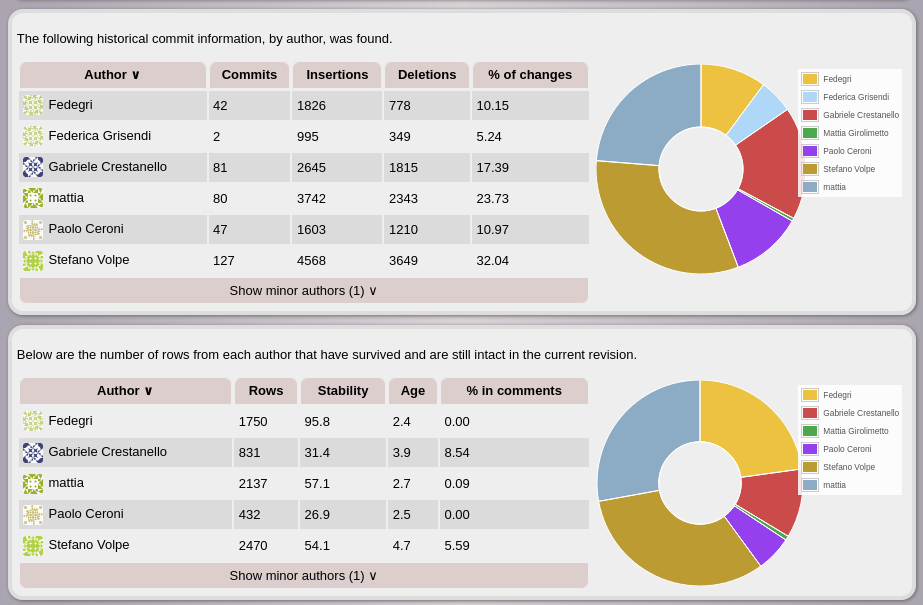
\includegraphics[width=\textwidth]{gitinspector.png}

\subsection{Retrospettiva finale con \emph{Essence}}

Dopo la retrospettiva dell'ultimo sprint, abbiamo effettuato una retrospettiva
generale per l'intero processo scrum. Ancora una volta, abbiamo scelto
\emph{Patience}, allo scopo di capire cosa ripetere e cosa evitare nei prossimi
progetti.

\includegraphics[width=\textwidth]{essence-final.jpg}

Dopo il successo della definizione di ``fatto'', la scoperta di una carta chiamata
\emph{Definition of Ready} è stata apprezzata in particolar modo dagli
sviluppatori. Questi hanno sostenuto che aggiungere tale pratica assicurerebbe
loro di inizare lo sprint solo con storie utente ragionevoli. Questo porterebbe
anche a un rapporto più equo fra PO e sviluppatori: così come gli sviluppatori
si sforzano di rispettare la definizione di fatto, il PO si sforza di
rispettare quella di pronto.

Se le carte Essence raccomandano team di sviluppo di 4 o 5 membri, è emerso il
desiderio di tentare di orientarsi verso un gruppo di 4 persone.

\subsection{Diagramma del \emph{deployment} del prodotto}

\includegraphics[width=\textwidth]{deployment.png}

\section{Demo}

Un video che illustra l'uso del prodotto è disponibile
\underline{\href{https://liveunibo-my.sharepoint.com/:v:/g/personal/federica_grisendi_studio_unibo_it/EaOojpKKw9ZIreuXeDcHFicBxvcOjSGP4zPOGXMwKPtEcA?e=QVfOKm}{a questo indirizzo}}.

\section{Artefatti}

\begin{itemize}
	\item API: \url{http://team13.hjkl.gq:8000/swagger/index.html}
	\item frontend web: \url{http://team13.hjkl.gq/}
\end{itemize}

\end{document}
